\documentclass[12pt]{article}
\linespread{1.3}
\usepackage{hyperref}
\usepackage{enumitem}
%\usepackage{enumerate}
\usepackage{changepage,lipsum,titlesec, longtable}
\usepackage{cite}
\usepackage{comment, xcolor}
\usepackage[pdftex]{graphicx}
  \graphicspath{{images/}, {images/stat/}}
  \DeclareGraphicsExtensions{.pdf,.jpeg,.png, .jpg}
\usepackage[cmex10]{amsmath}
\usepackage{tikz}
\usepackage{array} 
\usepackage{subfigure} 
\newcommand{\grey}[1]{\textcolor{black!30}{#1}}
\newcommand{\red}[1]{\textcolor{red!50}{#1}}
\newcommand{\question}[1]{\textcolor{magenta}{\textbf{Question: } {#1}}}
\newcommand{\fref}[1]{Figure~\ref{#1}}
\newcommand{\tref}[1]{Table~\ref{#1}}
\newcommand{\eref}[1]{Equation~\ref{#1}}
\newcommand{\cref}[1]{Chapter~\ref{#1}}
\newcommand{\sref}[1]{Section~\ref{#1}}
\newcommand{\aref}[1]{Appendix~\ref{#1}}
\newcommand{\note}[0]{\textbf{Note: }}

\renewcommand{\labelenumii}{\theenumii}
\renewcommand{\theenumii}{\theenumi.\\arabic{enumii}.}

\oddsidemargin0cm
\topmargin-2cm %I recommend adding these three lines to increase the
\textwidth16.5cm %amount of usable space on the page (and save trees)
\textheight23.5cm

\makeatletter
\renewcommand\paragraph{\@startsection{paragraph}{4}{\z@}%
            {-2.5ex\@plus -1ex \@minus -.25ex}%
            {1.25ex \@plus .25ex}%
            {\normalfont\normalsize\bfseries}}
\makeatother
\setcounter{secnumdepth}{4} % how many sectioning levels to assign numbers to
\setcounter{tocdepth}{4}    % how many sectioning levels to show in ToC

% draw diagram
\usetikzlibrary{shapes.geometric, arrows}
\tikzstyle{data} = [font=\scriptsize, rectangle, rounded corners, minimum width=1.5cm, minimum height=1cm,align=left, draw=black, fill=black!30]
\tikzstyle{database} = [font=\scriptsize, rectangle, rounded corners, minimum width=3cm, minimum height=1cm,align=left, draw=black, fill=green!30]
\tikzstyle{query} = [font=\scriptsize,trapezium, trapezium left angle=70, trapezium right angle=110, minimum width=0.5cm, minimum height=0.5cm, text centered, draw=black, fill=blue!30]
\tikzstyle{process} = [font=\scriptsize,rectangle, minimum width=3cm, minimum height=1cm, text centered, draw=black, fill=orange!30]
\tikzstyle{spliter} = [font=\scriptsize,diamond, minimum width=2cm, minimum height=1cm, text centered, draw=black, fill=green!30]
\tikzstyle{decision} = [font=\scriptsize,diamond, minimum width=3cm, minimum height=1cm, text centered, draw=black, fill=green!30]
\tikzstyle{arrow} = [thick,->,>=stealth]
\tikzstyle{bi-arrow} = [thick,->,>=stealth]


\begin{document}
\title{New GSA data process and weather normalization\\
       \large GSA project}
\maketitle
\tableofcontents
\newpage
\section{Question}\label{sec:ques}
Weather normalization: is it only weather or both weather and climate
\section{Terms}
\begin{description}
\item[Heating balance-point temperature] The temperature above which
no thermal energy is needed for space heating.
\end{description}
\section{Introduction}\label{sec:intro}
The document records the literature search of weather
normalization. The weather normalization, as described in the
\href{https://portfoliomanager.energystar.gov/pdf/reference/Climate%20and%20Weather.pdf}{PM
  EnergyStar Technical Reference}, ``is the energy your building
would have used under average conditions (also referred to as climate
normals)''. The difference of weather condition each year can affect
the energy consumption of a building, taking this influence into
account is the reason for weather normalization. As is mentioned in
the document, ``the normalization process is performed separately for
each fuel that is present (electricity, gas, district steam, etc.)''

Climate normals could be obtained from \url{http://www.ncdc.noaa.gov/oa/climate/normals/usnormals.html}

\section{Common Method}
\subsection{Energy Star method}
The document of \href{https://portfoliomanager.energystar.gov/pdf/reference/Climate%20and%20Weather.pdf}{Energy Star Portfolio Manager} has the following steps.
\begin{enumerate}
\item Retrieve 24 (or at least 12) calendar months of energy data.
\item Plotting energy-temperature (energy is y axis), a plot is
  created for each type of energy fuel
\item Using linear regressions to calculate the fit line maximizing
  the $R^2$, after this step one gets a function maps from temperature
  to energy consumption of some fuel $$F: T \mapsto E$$ where $T$:
  temperature and $E$: energy This step is the trickiest one, the
  following document would describe this step in more detail.
\item Compute the ratio $$r = {F(T_{normal}) \over F(T_{current})}$$
  where $T_{normal}$ is 
\item Compute normalized energy: $$E_{norm} = r \cdot E_{current}$$
\end{enumerate}
In the steps above, the step 3 is not very clear on the regression
computing process.  From other technical document, the model uses HDD
or CDD as the independent variable (input to the function) in
regression computation: ``ENERGY STAR model is a amount of raw fuel
regression-based model that builds on the PRISM approach by using that
is required to degree-day models.''~\cite{LEAN2013}. Some other
independent variables such as occupancy and equipment are also
included. The dependent variable is the source EUI. The HDD and CDD
are retrieved by Zip code.

\subsection{LEAN Energy Analysis, Using Regression Analysis to
Assess Building Energy Performance}
LEAN analysis uses monthly bills, gross or conditioned area, building
typology and current and normal weather data.
The steps are as follows:
\begin{enumerate}
\item For each energy usage type, create a regression model of energy
  vs. weather condition. The model has three parameters: base load,
  ``weather dependent energy use'', and ``balance point''.
\item Use historical energy and weather data to build a historical
  model.
\item Use recent energy and weather data to build a current model
\end{enumerate}
\red{Seems very confusing, what is the first step doing?}
\subsection{PRISM Method}
``The PRISM ® (PRInceton Scorekeeping Method) is one of the earliest
applications of using regression analysis to measure energy savings in
commercial buildings.''~\cite{LEAN2013}, this method computes a
``weather adjusted index of energy consumption'' from 12 month of
energy consumption data.
\subsection{Inverse Model Toolkit by ASHRAE}
This document is cited by \cite{LEAN2013}, describing how to build the
regression model.

The model uses a generalized least square regression.

There are several models described in the document
\subsubsection{Variable-based degree-day model} 
It is used for single zone buildings, in this model, the IMT searches
the balance that maximizes $R^2$ as follows:
  \begin{figure}[h!]
    \centering
    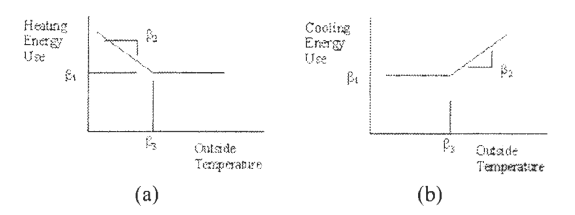
\includegraphics[width=0.7\linewidth]{singleZone.png}
    \caption{Single zone building energy use patterns}
  \end{figure}
  Take heating for example: IMT VBDD model is defined as
  $$Y = \beta_1 + \beta_2 HDD(\beta_3)$$
  where $HDD(\beta_3)$ is the heating degree days with $\beta_3$ as
  the base temperature. Monthly degree days with different base
  temperature is calculated and stored in a table. Each row is one
  month and each column has a different base temperature. In the
  document the base temperature search range is 41 F to 80 F. However
  I propose to search within the range of [40, 45, 50, 55, 57, 60, 65]
  for HDD and [45, 50, 55, 57, 60, 65, 70, 72] for CDD for weather
  normalization usage, since one need to acquire a corresponding
  climate normal with the same base temperature, and these are the
  available base temperature for climate normal in NCDC. For the HDD
  example, the algorithm will compute a regression line for each base
  temperature in the search range and return the regression line with
  the maximum $R^2$

\subsubsection{Change point model}
In VBDD model, the assumption is when the ambient temperature is above
heating base temperature or below cooling base temperature (the one
used to calculate HDD or CDD), energy will not change with ambient
temperature. Change-point (CP) models remove this assumption and
account for energy change throughout the ambient temperature range. It
also accounts for the non-linear relationship between heating /
cooling energy consumption and the ambient temperature.

\subsection{ASHRAE Guideline 14}
\subsection{IPMVP Volume I}
\section{Weather data}
Might be available from
\url{http://www.wunderground.com/history/airport/KTUS/2012/1/22/MonthlyHistory.html?req_city=Pittsburgh&req_state=PA&req_statename=Pennsylvania&reqdb.zip=15217&reqdb.magic=1&reqdb.wmo=99999}
\newpage
\bibliographystyle{plain} \bibliography{myCitation}
\end{document}